\documentclass[fleqn,12pt]{article}

\usepackage[utf8]{inputenc}
\usepackage[T1]{fontenc}
\usepackage{mathtools} %loads amsmath
\usepackage{amsthm}
\usepackage{amsfonts}
\usepackage{amsmath}
\usepackage{amssymb}
\usepackage{graphicx}
\usepackage{tikz}
\usetikzlibrary{arrows,automata,positioning}
\usepackage{arydshln}
\usepackage{stmaryrd}
\usetikzlibrary{arrows,automata}
\usepackage{ stmaryrd }

\usepackage{fancyhdr}
\setlength{\headheight}{26pt}
\pagestyle{fancy}
\lhead{Static Program Analysis WS 2016/17 -- Series 02 \\ \small{Igor Dudschenko (296764)}, \small{Oliver Westphal (358321)}}
\rhead{}

\newcommand\dbrackets[1]{\llbracket #1 \rrbracket}

\setlength{\parindent}{0cm}
\newcommand\note[1]{\textcolor{red}{#1}}

\begin{document}
\section*{Exercise 1}
To disprove the soundness of the introduced transfer function:
$$\Phi (V) := (V \cup gen_{LV}(B^{l'}) \setminus  kill_{LV}(B^{l'})$$
we used the example from the lecture (see Fig. \ref{fig:lecEx}) and observed changes in the LV equation system, thus the transfer function cannot be sound:
$$LV_1 = \Phi_2(LV_2) = LV_2 \setminus \{ y \}$$
$$LV_2 = \Phi_3(LV_3) = LV_3 \setminus \{ x \}$$
$$LV_3 = \Phi_4(LV_4) = LV_4 \cup \{ y \}$$
$$LV_4 = \Phi_5(LV_5) =( LV_5 \cup \{ x \}) \setminus \{ z \}$$
$$LV_5 = \Phi_6(LV_6) =( LV_6 \cup \{ y \}) \setminus \{ z \}$$
$$LV_6 = \Phi_7(LV_7) =( LV_7 \cup \{ z \}) \setminus \{ x \}$$
$$LV_7 = \{x,y,z\}$$
Unique Solutions:
$$LV_1 = \emptyset$$
$$LV_2 =  \{ y \}$$
$$LV_3 =  \{ x, y \}$$
$$LV_4 =  \{ x, y \}$$
$$LV_5 =  \{  y \} \neq \{ x, y \} \lightning$$
$$LV_6 =  \{  y, z \}$$
$$LV_7 =  \{  x, y, z \}$$
\begin{figure}[!htb]
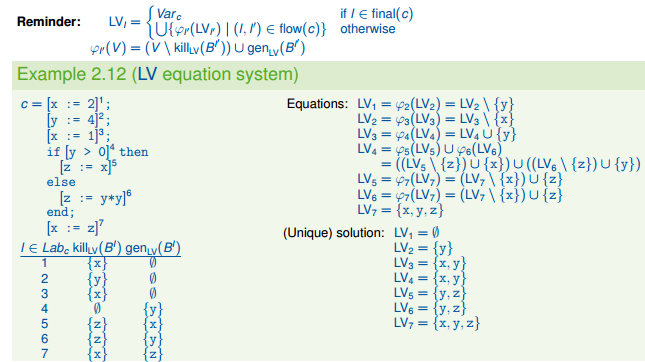
\includegraphics[width=\textwidth,keepaspectratio]{LectureExample.png}
\caption{Live Variable Analysis, this example was introduced during the Lecture.}
\label{fig:lecEx}
\end{figure}
\section*{Exercise 2}
\subsection*{(a)}
\includegraphics[]{lattice.pdf}
%For $l \in final(c):$
%\begin{center}
%$$\top = LV_l = Var_c = \{x, y, z\}$$
%$$\downarrow$$
%$$LV_{l-1}$$
%$$\downarrow$$
%$$.$$
%$$.$$
%$$.$$
%$$\downarrow$$
%$$LV_{l-l+11}$$
%$$\downarrow$$
%$$LV_{0} = \emptyset = \bot$$
%\end{center}
\subsection*{(b)}
Every connected graph with a common source and a common sink is a valid lattice. Common source means there exists only one node that has no incoming edges and common sink means there exists only one node with no outgoing edges. Graphs 1,2,4 and 6 are valid lattices. Graph 3 has two nodes with no outgoing edges and thus has no %Greater Lower Bound.
uniqe least element Graph 5 has neither %Greater Lower Bound
a uniqe least element nor a Least Upper Bound for every subset. Check Figure \ref{fig:graphs} for enumeration.

\begin{figure}[!htb]
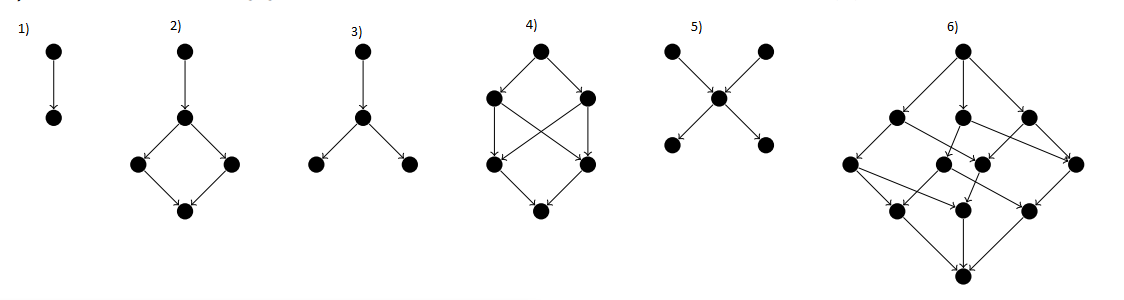
\includegraphics[width=\textwidth,keepaspectratio]{Graphs.png}
\caption{Exercise 2b - Lattice Graphs}
\label{fig:graphs}
\end{figure}

\section*{Exercise 3}
\subsection*{(a)}
%\textbullet There is no modification required for $( \mathbb{Z}_{\geq 0},\geq )$, since it has a Least Upper Bound (in this case it is 0) and eventually always stabilises.\\
%\textbullet Since A is downward closed, S has to have a Least Upper Bound and therefore it is satisfying ACC. The height of of S is not bounded by by any k, since the set is infinitely large.
\textbullet $( \mathbb{Z}_{\geq 0},\geq )$ should be modified to $( \{ n | n \in \mathbb{Z}_{\geq 0}, a \geq n \},\geq )$ for some arbitray but fixed $a$.
Otherwise there is no least element $\perp = \sqcup \emptyset$ and also there would exist ascending chains which do not stabilise, since they can start arbitrarily "low" w.r.t. $\geq$.\\
\textbullet $(S,\subseteq)$ is isomorphic to $(\mathbb{N},\leq)$, which arcording to the lecture does not satisfy ACC nor has it bounded height.
\subsection*{(b)}
%A lattice consisting of finite chains always has a Least Upper Bound and thus is a complete lattice and therefore it also has the ACC properties.
Since an ascending chain only consists of elements from a single chain from the lattice, the fact that each chain is finite implies every ascending chain contains only finitely many distinct elements.
Therefore every ascending chain must stabilize, so by definition ACC holds.
\section*{Exercise 4}
\subsection*{(a)}

\subsection*{(b)}

\subsection*{(c)}

\subsection*{(d)}

\end{document}